\section{Haar-Cascade}\label{sec:haar-cascade}

Método cascade há um conjunto de imagens, as que contém as características que se deseja extrair (imagens positivas) e as que não tem correspondência com o que deseja (imagens negativas). Um exemplo seria com a detecção facial. Haveria um conjunto de imagens de faces, positivas, e outras que não fossem faces, negativas.

%\begin{comment}

\begin{figure}[ht]
\centering
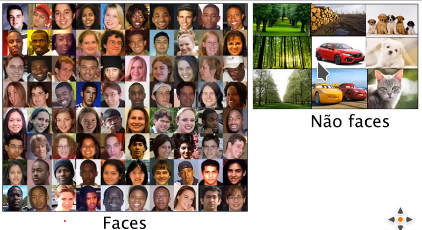
\includegraphics[width=8cm]{images/cascade.png}
\caption{Exemplos de faces usadas pelo cascade}
\label{fig:cascade}
\end{figure}

%\end{comment}

Logo após um treinamento de imagens é feito com o algoritmo AdaBoost. E por seguinte é selecionado os melhores conjuntos de características. A característica é dada pela soma dos pixels que se situam dentro dos retângulos brancos e são subtraídos da soma dos pixels em retângulos em cor cinza segundo Viola e Jones (2001). Então, esse resultado irá representar o valor encontrado pela característica para determinada região \cite{refer4}.

Ao tentar identificar um rosto seja em uma foto ou um vídeo, é feito a busca pixel por pixel até encontrar características que sejam correspondente. 

A partir da integral de imagem é possível identificar padrões utilizando características Haar-like, que são máscaras retangulares nas quais os valores dos pixels de uma região são subtraídos dos valores dos pixels de outra região, representando uma diferença de intensidade luminosa entre áreas da imagem. 
O algoritmo é dividido em três partes:
A criação da imagem integral, a representação da imagem em um espaço de características baseados nos filtros de Haar.

Montagem de um classificador de aprendizado Boosting chamado de AdaBoost, capaz de selecionar as características relevantes.

Criação de uma estrutura em árvore, chamada cascata de classificadores.
